% =====================================================================
%  fig01 — Process & global-catastrophe schematic
%  Two-type birth--death--conversion process with a single global
%  absorbing catastrophe entered at total rate  delta_1 x + delta_2 y.
%
%  Orientation figure for Sections 1--2 of
%  "Type-specific catastrophe hazards in a two-type branching process".
%
%  Vector schematic.  Build:  pdflatex fig01.tex   (-> fig01.pdf)
%  Notation and rates follow sections/02_model.tex exactly.
% =====================================================================
\documentclass[tikz,border=10pt]{standalone}

\usepackage[T1]{fontenc}
\usepackage{lmodern}          % match the paper's Latin Modern math
\usepackage{amsmath,amssymb,mathtools}
\usepackage{xcolor}

\usetikzlibrary{arrows.meta,positioning,calc,backgrounds,fit}

% ---- paper macro (absorbing catastrophe state) ----------------------
\newcommand{\R}{\mathsf R}

% ---- palette (SHARED_CONVENTIONS.md) --------------------------------
\definecolor{type1}{HTML}{0072B2}   % type 1  (primary blue)
\definecolor{type2}{HTML}{D55E00}   % type 2  (vermillion)
\definecolor{cata}{HTML}{9A2820}    % catastrophe sink (soft red)
\definecolor{ink}{HTML}{1A1C1F}     % near-black
\definecolor{inksoft}{HTML}{565B62} % secondary text
\definecolor{rule}{HTML}{E3E6EA}    % very light rules
\definecolor{type1fill}{HTML}{E9F1F8}
\definecolor{type2fill}{HTML}{FBEEE5}
\definecolor{cardfill}{HTML}{F8FAFC}
\definecolor{pillfill}{HTML}{FFFFFF}

\begin{document}
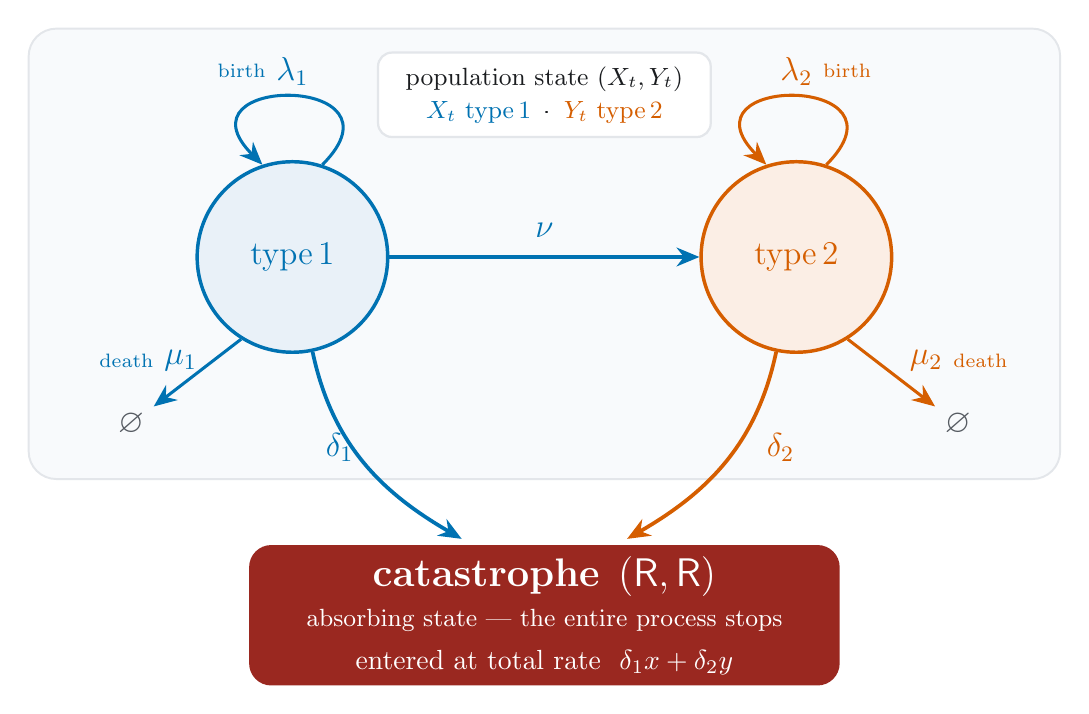
\begin{tikzpicture}[
    >={Stealth[length=2.9mm,width=2.4mm]},
    font=\normalsize,
    % --- individual nodes -------------------------------------------
    indiv/.style={circle,minimum size=2.42cm,line width=1.25pt,
                  inner sep=0pt,align=center,font=\large},
    t1/.style={indiv,draw=type1,fill=type1fill,text=type1},
    t2/.style={indiv,draw=type2,fill=type2fill,text=type2},
    % --- event arrows ------------------------------------------------
    ev1/.style={draw=type1,line width=1.1pt,->},
    ev2/.style={draw=type2,line width=1.1pt,->},
    haz1/.style={draw=type1,line width=1.35pt,->},
    haz2/.style={draw=type2,line width=1.35pt,->},
    % --- rate labels -------------------------------------------------
    rlab1/.style={text=type1,font=\large,inner sep=1.5pt},
    rlab2/.style={text=type2,font=\large,inner sep=1.5pt},
    % --- misc --------------------------------------------------------
    empt/.style={inksoft,font=\large},
    soft/.style={text=inksoft},
  ]

% =====================================================================
%  Geometry (centimetres)
% =====================================================================
\coordinate (T1) at (0,0);
\coordinate (T2) at (6.4,0);

% ---- soft "local events" card (background layer) --------------------
\begin{scope}[on background layer]
  \fill[cardfill,rounded corners=10pt] (-3.35,-2.82) rectangle (9.75,2.90);
  \draw[rule,line width=0.7pt,rounded corners=10pt] (-3.35,-2.82) rectangle (9.75,2.90);
\end{scope}

% =====================================================================
%  Population-state pill  (upper centre, inside card)
% =====================================================================
\node[draw=rule,fill=pillfill,rounded corners=5pt,line width=0.8pt,
      inner xsep=10pt,inner ysep=5pt,font=\small,text=ink,align=center] at (3.2,2.06)
     {population state $(X_t,Y_t)$\\[1pt]
      \textcolor{type1}{$X_t$ type\,1}\ \,·\,\ \textcolor{type2}{$Y_t$ type\,2}};

% =====================================================================
%  Individual nodes
% =====================================================================
\node[t1] (n1) at (T1) {type\,1};
\node[t2] (n2) at (T2) {type\,2};

% ---- birth self-loops (self-replication cue) ------------------------
\draw[ev1] (n1.72) to[out=45,in=135,looseness=5.5] (n1.108);
\node[rlab1] (lam1) at (0,2.36) {$\lambda_1$};
\node[rlab1,font=\scriptsize,anchor=east,inner sep=2pt] at (lam1.west) {birth};
\draw[ev2] (n2.72) to[out=45,in=135,looseness=5.5] (n2.108);
\node[rlab2] (lam2) at (6.4,2.36) {$\lambda_2$};
\node[rlab2,font=\scriptsize,anchor=west,inner sep=2pt] at (lam2.east) {birth};

% ---- conversion  type1 -> type2  (irreversible) ---------------------
\draw[ev1] (n1.east) -- (n2.west);
\node[rlab1] at (3.2,0.34) {$\nu$};

% ---- ordinary deaths -> empty set (local) ---------------------------
\node[empt] (d1) at (-2.05,-2.12) {$\varnothing$};
\draw[ev1] (n1.238) -- (d1);
\node[rlab1] (mu1) at (-1.42,-1.32) {$\mu_1$};
\node[rlab1,font=\scriptsize,anchor=east,inner sep=2pt] at (mu1.west) {death};

\node[empt] (d2) at (8.45,-2.12) {$\varnothing$};
\draw[ev2] (n2.302) -- (d2);
\node[rlab2] (mu2) at (8.05,-1.32) {$\mu_2$};
\node[rlab2,font=\scriptsize,anchor=west,inner sep=2pt] at (mu2.east) {death};

% =====================================================================
%  Catastrophe hazard arrows (colour-coded contributions) -> sink
% =====================================================================
\draw[haz1] (n1.282) to[out=-78,in=150] (2.15,-3.58);
\node[rlab1] at (0.60,-2.42) {$\delta_1$};
\draw[haz2] (n2.258) to[out=-102,in=30] (4.25,-3.58);
\node[rlab2] at (6.20,-2.42) {$\delta_2$};

% =====================================================================
%  Global absorbing catastrophe sink
% =====================================================================
\node[rectangle,rounded corners=8pt,fill=cata,text=white,
      minimum width=7.5cm,minimum height=1.72cm,align=center,
      inner sep=4pt] (sink) at (3.2,-4.55)
     {{\Large\bfseries catastrophe}\ \ {\Large\bfseries $(\R,\R)$}\\[2.5pt]
      {\small absorbing state --- the entire process stops}\\[3.5pt]
      {\normalsize entered at total rate\ \ $\delta_1 x+\delta_2 y$}};

\end{tikzpicture}
\end{document}
